\documentclass{letter}
\usepackage[english]{babel}
\usepackage{graphicx,alltt}

%%%%%%%%%% Start TeXmacs macros
\newcommand{\paragraph}[1]{\smallskip--\noindent\textbf{#1}}
\newcommand{\tmem}[1]{{\em #1\/}}
%%%%%%%%%% End TeXmacs macros

\begin{document}

\title{Wavelets}

\author{Martino Ferrari}

\maketitle

\subsubsection{Introduction}\label{introduction}

\paragraph{Exercise 1.1}\label{exercise-1.1}

Give a manual decomposition of $g (x) = [9, 7, 3, 5]$ in 2 scales.

First we perform a mean, representing the low frequency component:
\[ g_{\mu_1} (x) = \frac{9 + 7}{2}, \frac{3 + 5}{2} = [8, 4] \]
Then we can compute the {\tmem{high frequency}} component:
\[ g_{d_1} (x) = 9 - 8, 3 - 4 = [1, - 1] \]
Then the decoposiotion is represented by the two vectors:
\[ d_1 = [8, 4 ; 1, - 1] \]
We can applay the same operation to compute the decomposition at the second
scale:
\[ g_{\mu_2} (x) = \frac{8 + 4}{2} = [6] \]
\[ g_{d_2} (x) = 8 - 6 = 2 \]
\[ d_2 = [6 ; 2 ; 1, - 1] \]
\paragraph{Exercise 1.2}\label{exercise-1.2}

Given the Discrete Wavelet Transform at scale 3:
\[ d_3 = [36, 11, 22, 9, 2, 0, 2, 0] \]
\[ d_3 [1] = \frac{d_2 [1] + d_2 [2]}{2} \]
\[ d_3 [2] = d_2 [1] - d_3 [1] = d_2 [1] - \frac{d_2 [1] + d_2 [2]}{2} \]
Compute the inverse transformation $f'$:
\[ d_2 [1] = d_3 [2] + d_3 [1] \]
\[ d_2 [2] = d_3 [1] \cdot 2 - d_2 [1] = d_3 [1] - d_3 [2] \]
And so we can compute:
\[ d_2 = [36 + 11, 36 - 11, 22, 9, 2, 0, 2, 0] = [47, 25, 22, 9, 2, 0, 2, 0]
\]
Then
\[ d_1 = [47 + 22, 47 - 22, 25 + 9, 25 - 9, 2, 0, 2, 0] = [69, 25, 34, 16, 2,
   0, 2, 0] \]
And finally:
\[ f' = [69 + 2, 69 - 2, 25, 25, 34 + 2, 34 - 2, 16, 16] = [71, 67, 25, 25,
   36, 32, 16, 16] \]
Due to the fact that the negative components of $d_3$ were lost the
riconstruction is not perfect (yet similar).

\begin{figure}[h]
  \begin{center}
    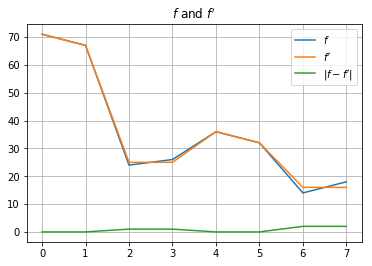
\includegraphics{output_5_0.png} 
  \end{center}
  \caption{png}
\end{figure}

\subsubsection{The 1D Haar Wavelet}\label{the-1d-haar-wavelet}

\paragraph{Exercise 2.1}\label{exercise-2.1}

Draw all box functions for vector-space $V_0$ and $V_1$:

\begin{figure}[h]
  \begin{center}
    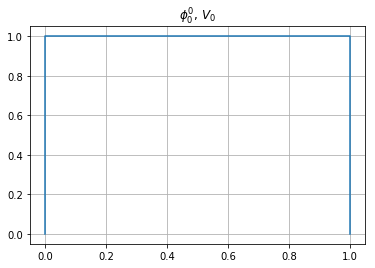
\includegraphics{output_7_0.png} 
  \end{center}
  \caption{png}
\end{figure}

\begin{figure}[h]
  \begin{center}
    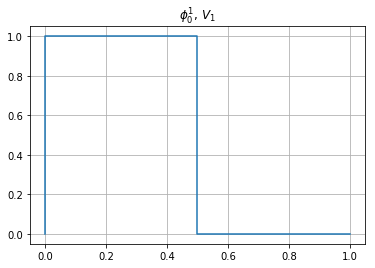
\includegraphics{output_7_1.png} 
  \end{center}
  \caption{png}
\end{figure}

\begin{figure}[h]
  \begin{center}
    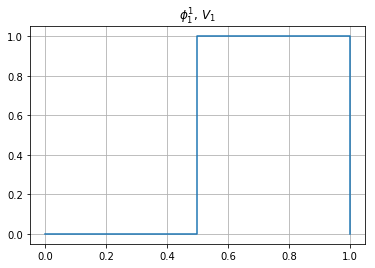
\includegraphics{output_7_2.png} 
  \end{center}
  \caption{png}
\end{figure}

\paragraph{Exercise 2.2}\label{exercise-2.2}

Give the normalized coefficients of the Haar wavelet decomposition of $f (x)$
into $V_0$, $W_0$ and $W_1$:
\[ \phi^0_0 (x) = 1 \phi (x) \]
\[ \psi^0_0 (x) = 1 \psi (x) \]
\[ \psi^1_0 (x) = \sqrt{2} \psi (2 x) \]
\[ \psi^1_1 (x) = \sqrt{2} \psi (2 x - 1) \]
\begin{figure}[h]
  \begin{center}
    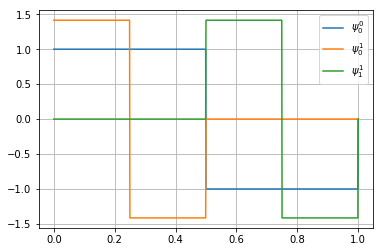
\includegraphics{output_9_0.png} 
  \end{center}
  \caption{png}
\end{figure}

\subsubsection{Imaging}\label{imaging}

\paragraph{Exercise 3.1}\label{exercise-3.1}

In this exercise I computed the {\tmem{dwt}} transform of
{\tmem{Cameraman.bmp}} and display the four components:

\begin{figure}[h]
  \begin{center}
    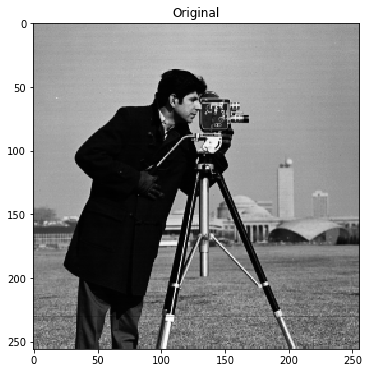
\includegraphics{output_11_0.png} 
  \end{center}
  \caption{png}
\end{figure}

\begin{figure}[h]
  \begin{center}
    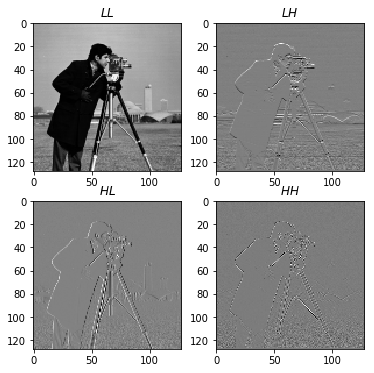
\includegraphics{output_11_1.png} 
  \end{center}
  \caption{png}
\end{figure}

\paragraph{Exercise 3.2}\label{exercise-3.2}

Using the function {\tmem{wavedec}} is possible to compute the wavelet
decomposition of the image. After computing the components we were asked to
order it by magnetude:

\begin{figure}[h]
  \begin{center}
    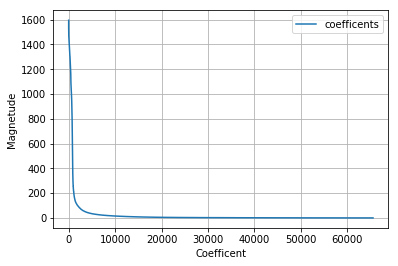
\includegraphics{output_13_0.png} 
  \end{center}
  \caption{png}
\end{figure}

Is very interesting to see that few components have most of the energy and
information (around 10000) whil the most of the others have magentude around
0.

\paragraph{Exercise 3.3}\label{exercise-3.3}

Using the information gatered previously I was able to compress (by nullify
the value of some components) the image. To do so first I decomposed the
image, than I nullify each component lower than a fixed treshold $\tau$ that I
fixed to 10 (after few tests):
\begin{alltt}

Treshold: 10
percentual of zeros: 79.20%
PSNR: 39.36
MSE: 7.541

\end{alltt}
\begin{figure}[h]
  \begin{center}
    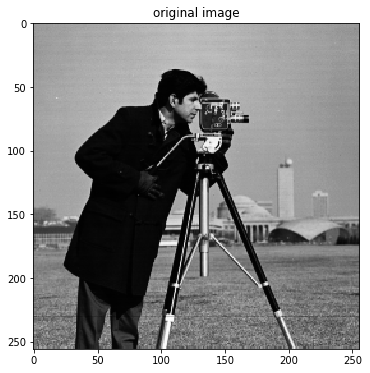
\includegraphics{output_15_1.png} 
  \end{center}
  \caption{png}
\end{figure}

\begin{figure}[h]
  \begin{center}
    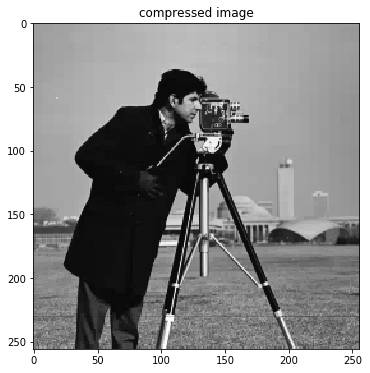
\includegraphics{output_15_2.png} 
  \end{center}
  \caption{png}
\end{figure}

\begin{figure}[h]
  \begin{center}
    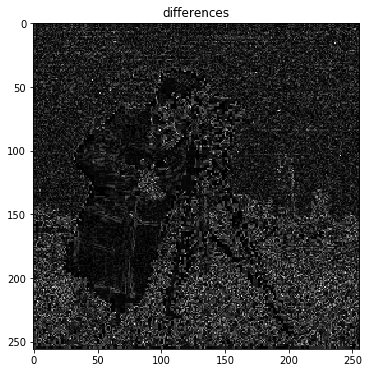
\includegraphics{output_15_3.png} 
  \end{center}
  \caption{png}
\end{figure}

The results is very interesting, the recostructed image is very close to the
original, with a $MSE = 7.761$ and a $PSNR = 39.23$. As possible to see in the
previous figure the differnece is as well very small and mostly concented on
the high-frequency areas.

To understand better the quality and capacity of the compression I chose to
variate the treshold from 1 to 1600 (with a step of 10) and plot the results:

\begin{figure}[h]
  \begin{center}
    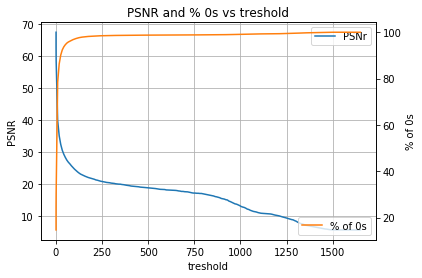
\includegraphics{output_18_0.png} 
  \end{center}
  \caption{png}
\end{figure}

\begin{figure}[h]
  \begin{center}
    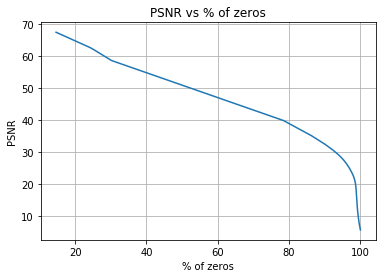
\includegraphics{output_18_1.png} 
  \end{center}
  \caption{png}
\end{figure}

In the fist figure I plotted the {\tmem{PSNR}} and the percentage of nullified
components against the treshold. The percentage of zeros reach values close to
the 100\% very quickly and at the same time the {\tmem{PSNR}} decrease at
frist very quiclky and then more linearly. With a treshold

For this reason the second plot is porbably more interesting as instead of
using the treshold as $x$ axis I used the pecentage of zeros.

In this way is possible to see that the {\tmem{PSNR}} decrease linearly with
the percentage of zeros (as both have similar trend in the against the
threshold) till 90\% and the implode quickly.

This results is very good, as it told us that even with high compression
80-90\% we can get a good quality image. However I'm expecting some kind phase
transition close to 0\% of zeros to visualize it I chose to focus on the
trehold range $\tau \in [0, 0.5]$:

\begin{figure}[h]
  \begin{center}
    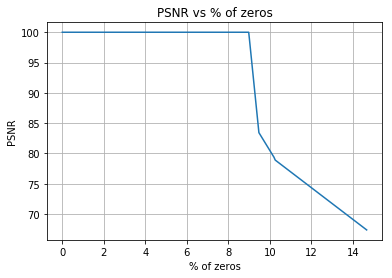
\includegraphics{output_21_0.png} 
  \end{center}
  \caption{png}
\end{figure}

As expected with few percentage of zeros there is no relevant loss of
information. The decrease of quality in the picture starts only from around
9\% of zeros.

\end{document}
